\newpage
\section{Resultados}

\newcommand{\graficoreservado}[3]{%
\begin{figure}[H]
    \centering
    \caption{#1}
    \label{#2}
    \vspace{0.3cm}
    \fbox{\parbox[c][4.2cm][c]{0.85\textwidth}{\centering Espaço reservado para o gráfico\\ #3}}
    \vspace{0.2cm} \\
    Fonte: Autor.
\end{figure}}

\par Este capítulo apresenta os resultados e discute até que ponto confirmam os requisitos. A avaliação combina as medidas de desempenho com o sistema completo em contêineres, o ensaio de aquisição contra um servidor Modbus de teste e os ensaios na bancada com o inversor de frequência.

\subsection{Ambiente de ensaio}

\par As medidas foram obtidas no computador do autor, que fez o papel de servidor. Todos os processos executaram em contêineres \emph{Docker} \cite{DOCKER_DOCS}, com limites de processamento e de memória que reproduzem os recursos planejados, de modo que o teto medido seja o de um contêiner pequeno e não o da máquina inteira. O \emph{PostgreSQL} \cite{POSTGRESQL_DOCS} na versão 18 e o \emph{Redis} \cite{REDIS_DOCS} na versão 8 também executaram em contêineres. A Tabela~\ref{tab:cap7_ambiente} resume o equipamento e as versões, e a Tabela~\ref{tab:cap7_limites} lista os limites.

{\renewcommand{\arraystretch}{1.3}\small
\begin{xltabular}{\textwidth}{lX}
        \caption{Ambiente de ensaio.}
        \label{tab:cap7_ambiente}\\
        \hline
        \textbf{Item} & \textbf{Descrição} \\
        \hline
        \endfirsthead
        \hline
        \textbf{Item} & \textbf{Descrição} \\
        \hline
        \endhead
        \endfoot
        \multicolumn{2}{c}{Fonte: Autor.} \\
        \endlastfoot
        Computador (servidor) & Intel Core i5-13420H com 12 \emph{threads}, cerca de 32\,GB de memória, Windows 11 Pro \\
        \hline
        Virtualização & Docker Desktop com máquina virtual de 4 processadores lógicos e 6\,GB de memória durante a campanha de capacidade \\
        \hline
        Banco de dados & PostgreSQL 18.6 em contêiner \\
        \hline
        Cache, filas e transporte & Redis 8.10 em contêiner, com política \emph{noeviction} \\
        \hline
        Aplicação & Node.js 24, imagens de produção construídas em estágios, uma por serviço \\
        \hline
        Dispositivo de campo simulado & Simuladores Modbus, um do próprio repositório, com milhares de \sigla{clp} virtuais, e o ProtoProbe do autor (porta 502, escravo 1) \\
        \hline
\end{xltabular}}

{\renewcommand{\arraystretch}{1.3}\small
\begin{xltabular}{\textwidth}{lccX}
        \caption{Limites de recursos dos contêineres.}
        \label{tab:cap7_limites}\\
        \hline
        \textbf{Contêiner} & \textbf{Processamento} & \textbf{Memória} & \textbf{Observação} \\
        \hline
        \endfirsthead
        \hline
        \textbf{Contêiner} & \textbf{Processamento} & \textbf{Memória} & \textbf{Observação} \\
        \hline
        \endhead
        \endfoot
        \multicolumn{4}{c}{Fonte: Autor.} \\
        \endlastfoot
        API (Fastify) & 0,25 \emph{vCPU} & 512\,MB & Processo HTTP, sem \emph{workers} \\
        \hline
        \emph{Worker} & 0,25 \emph{vCPU} & 512\,MB & Um supervisor e um subprocesso por família de fila \\
        \hline
        Aquisição & 0,25 \emph{vCPU} & 512\,MB & Agendador e leitura Modbus, sem banco \\
        \hline
        Scripts isolados & 0,25 \emph{vCPU} & 512\,MB & Programa que executa os scripts, sistema de arquivos somente leitura \\
        \hline
        Web (Next.js) & 0,25 \emph{vCPU} & 512\,MB & Somente telas \\
        \hline
        Redis & 0,25 \emph{vCPU} & 1\,GB & \emph{maxmemory} de 512\,MB \\
        \hline
        PostgreSQL & 2 \emph{vCPU} & 1\,GB & \emph{shared\_buffers} de 256\,MB \\
        \hline
\end{xltabular}}

\par A soma dos limites é de 3,5 \emph{vCPU} e 4,5\,GiB. Um contêiner de 0,25 \emph{vCPU} para por alguns milissegundos ao esgotar sua cota de processamento, o que aparece no percentil 95, valor abaixo do qual ficam 95\,\% das medidas, e é uma característica do ambiente e não do código.

\par Cada degrau de carga roda dois ciclos de aquecimento, descartados, e doze ciclos medidos. Ele é sustentado quando pelo menos 99\,\% das leituras foram atendidas, o atraso no percentil 95 ficou abaixo de 20\,\% do período de varredura, as filas não cresceram na segunda metade da janela, nenhum contêiner reiniciou e o Redis ficou abaixo de 70\,\% da memória máxima. O teto é o maior degrau sustentado antes do primeiro reprovado.

\par A carga, o simulador de \sigla{clp}, o navegador e os contêineres dividem o mesmo computador, que executava também outras atividades, sem atraso de rede entre os contêineres. Os números, portanto, são de ordem de grandeza e valem como teto do servidor com equipamento que responde de imediato, e não como previsão para uma planta com modems lentos.

\subsection{Medidas de desempenho já realizadas}

\subsubsection{Desempenho das telas}

\par O desempenho das telas foi medido com o \emph{Lighthouse} em modo de celular, com rede e processador limitados, sobre a versão de produção e uma cópia isolada do sistema. Foram três execuções em cada tela, o sinótico, a lista de alarmes e o dashboard, e a Tabela~\ref{tab:cap7_lighthouse} apresenta a mediana, com o piso adotado como limite de regressão. O \emph{Largest Contentful Paint}, tempo até o maior elemento aparecer, ficou entre 1,25 e 1,51 s, abaixo do alvo de 2,5 s, e o deslocamento de \emph{layout} acumulado ficou muito abaixo do limite de 0,1. O tempo total de bloqueio da \emph{thread} principal foi maior no dashboard por causa do desenho dos gráficos.

{\renewcommand{\arraystretch}{1.3}\small
\begin{xltabular}{\textwidth}{Xccccccc}
        \caption{Resultados do \emph{Lighthouse} (celular), mediana de três execuções. Des.: desempenho, Ace.: acessibilidade, BP: boas práticas, LCP e TBT em ms.}
        \label{tab:cap7_lighthouse}\\
        \hline
        \textbf{Tela} & \textbf{Des.} & \textbf{Ace.} & \textbf{BP} & \textbf{SEO} & \textbf{LCP} & \textbf{CLS} & \textbf{TBT} \\
        \hline
        \endfirsthead
        \hline
        \textbf{Tela} & \textbf{Des.} & \textbf{Ace.} & \textbf{BP} & \textbf{SEO} & \textbf{LCP} & \textbf{CLS} & \textbf{TBT} \\
        \hline
        \endhead
        \endfoot
        \multicolumn{8}{c}{Fonte: Autor.} \\
        \endlastfoot
        Sinótico (execução) & 99 & 100 & 100 & 54 & 1.260 & 0 & 121 \\
        \hline
        Alarmes & 99 & 100 & 100 & 54 & 1.253 & 0,008 & 141 \\
        \hline
        Dashboard & 94 & 100 & 100 & 54 & 1.513 & 0,001 & 282 \\
        \hline
        Piso adotado & 94 / 94 / 89 & 95 & 95 & 49 & - & - & - \\
        \hline
\end{xltabular}}

\par A acessibilidade em 100 indica que o teste automático não encontrou violação das diretrizes \sigla{wcag}, o que não substitui a conferência com leitor de tela, que ficou como risco aceito. A pontuação de \emph{SEO} em 54 é esperada, porque a área com login é marcada como não indexável. As medidas apoiam os requisitos RNF12, RF13 e RF14.

\todo[inline]{As medianas vêm do registro de 15/10/2026 (madrugada) e o piso consta no CLAUDE.md do código com data de 14/10/2026. Confirmar qual data deve aparecer no texto e se vale citar o INP, que o Lighthouse não mede em modo de navegação.}

\par Mediu-se também o custo de atualizar um sinótico com 200 objetos, 120 vínculos e 506 nós gráficos, aberto por 60 s com dez tags mudando a cada ciclo. Nenhuma tarefa de mais de 50 ms foi registrada. O tempo para aplicar um ciclo de valores teve mediana de 6 ms e percentil 95 de 8 ms, abaixo dos 16 ms de um quadro a 60 quadros por segundo, o que sustenta os requisitos RNF01 e RF14.

\subsubsection{Motor de scripts isolado}

\par Variáveis derivadas, scripts e componentes de conteúdo executam em um motor isolado, como exige o RNF06. Com o programa que executa o motor (hospedeiro) já em funcionamento, em um contêiner de 0,25 \emph{vCPU}, o custo fixo de uma avaliação foi de 3,1 ms na mediana para a variável derivada, 3,5 ms para o script e 3,3 ms para o componente. O percentil 95 ficou entre 46 e 56 ms e o 99 entre 58 e 60 ms, valores que correspondem à pausa da cota de processador. O motor anterior, em \emph{Python}, custava cerca de 34 ms por avaliação, o que justificou a troca.

\par Um hospedeiro de 0,25 \emph{vCPU} sustentou de 144 a 149 avaliações por segundo, e quatro chegaram a 353. Por \emph{vCPU}, isso equivale a uma faixa de 380 a 590 avaliações por segundo, com ruído de cerca de 50\,\% entre execuções. O agrupamento em lote aumentou a vazão, como mostra a Figura~\ref{fig:cap7_lote}: com lote de 25, chegou-se em média a 545 avaliações por segundo, cerca de 3,7 vezes a de uma por vez.

\begin{figure}[H]
    \centering
    \caption{Vazão do motor de scripts em função do tamanho do lote, um hospedeiro de 0,25 \emph{vCPU}.}
    \label{fig:cap7_lote}
    \vspace{0.4cm}
    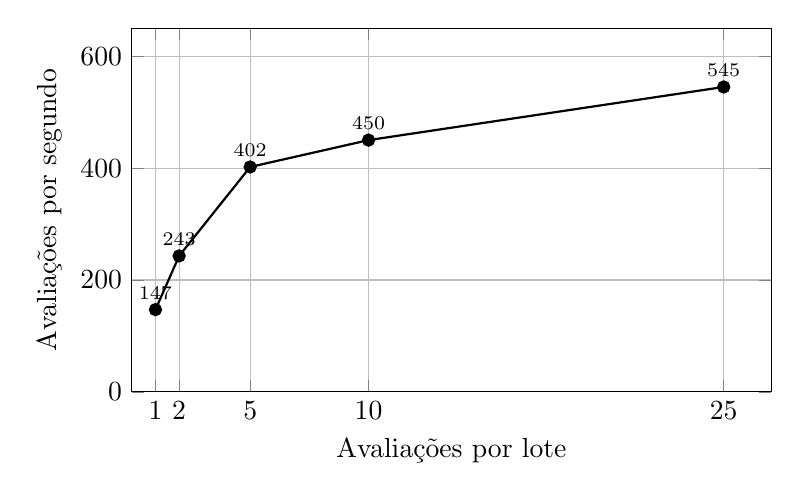
\begin{tikzpicture}
        \begin{axis}[
            width=0.8\textwidth, height=6.2cm,
            xlabel={Avaliações por lote},
            ylabel={Avaliações por segundo},
            xmin=0, xmax=27, ymin=0, ymax=650,
            xtick={1,2,5,10,25},
            grid=major,
            nodes near coords,
            every node near coord/.append style={font=\scriptsize, anchor=south},
        ]
            \addplot[mark=*, thick] coordinates {(1,147) (2,243) (5,402) (10,450) (25,545)};
        \end{axis}
    \end{tikzpicture}
    \vspace{0.2cm} \\
    Fonte: Autor.
\end{figure}

\par Esses resultados confirmam os requisitos RF11 e RF12.

\par O hospedeiro usou 17\,MiB de memória residente, e o contêiner dos scripts teve pico de 166\,MiB dos 512\,MiB permitidos. No contêiner de \emph{workers}, o pico foi de 435\,MiB, ou 85\,\% do limite, o mais apertado de todos, e a API chegou a 340\,MiB.

\par A Tabela~\ref{tab:cap7_meta} traz o teto sustentado de variáveis derivadas, chamadas de metas, e de tags internas geradas, comparado com o piso planejado. As metas liam duas tags e foram avaliadas de 1,2 a 1,85 vezes por ciclo, e as tags internas foram geradas em lotes de 25 por dispositivo. O primeiro recurso a saturar foi sempre o contêiner de \emph{workers}, e não o motor de scripts. As metas ficaram abaixo do piso a 5 e a 30 s e no piso a 10 s, e as tags internas ficaram abaixo do piso nas três faixas, o que levou a uma especificação dedicada à capacidade das filas de ingestão e de histórico.

{\renewcommand{\arraystretch}{1.3}\small
\begin{xltabular}{\textwidth}{lcccc}
        \caption{Teto sustentado de variáveis derivadas e de tags internas geradas por contêiner de 0,25 \emph{vCPU}.}
        \label{tab:cap7_meta}\\
        \hline
        \textbf{Carga} & \textbf{Período} & \textbf{Teto medido} & \textbf{Piso planejado} & \textbf{Alvo} \\
        \hline
        \endfirsthead
        \hline
        \textbf{Carga} & \textbf{Período} & \textbf{Teto medido} & \textbf{Piso planejado} & \textbf{Alvo} \\
        \hline
        \endhead
        \endfoot
        \multicolumn{5}{c}{Fonte: Autor.} \\
        \endlastfoot
        Variável derivada (meta) & 5 s & 50 & 150 & 450 \\
        \hline
        Variável derivada (meta) & 10 s & 250 & 250 & 750 \\
        \hline
        Variável derivada (meta) & 30 s & 150 & 1.000 & 3.000 \\
        \hline
        Tag interna gerada & 5 s & 100 & 350 & 1.050 \\
        \hline
        Tag interna gerada & 10 s & 350 & 525 & 1.575 \\
        \hline
        Tag interna gerada & 30 s & 250 & 2.800 & 8.400 \\
        \hline
\end{xltabular}}

\subsubsection{Gravação do histórico}

\par O histórico é gravado por uma fila própria, em lotes, numa tabela dividida por mês. O teste de carga mediu de 186 a 235 trabalhos por segundo com 40 linhas cada, ou 7.430 a 9.400 linhas por segundo, a um custo de 1,8 a 2,7 ms de processador por trabalho. A decisão de gravar, no Redis, custou 16,4 \textmu s por chamada e 2,3\,\% do processador do Redis a 1.000 leituras por segundo. A retirada de 200.000 linhas pelo expurgo levou 1,6 s, ou 125 mil linhas por segundo. Isso sustenta o RF02 com folga em relação à taxa de leitura da aquisição.

\par Outro teste manteve leituras contínuas por 10 minutos e conferiu que nenhuma tag ficava desatualizada na leitura final. Três execuções seguidas passaram, em 639, 652 e 636 s, o que confirma o RF03.

\subsection{Aquisição e ensaio com o simulador}

\subsubsection{Capacidade de leitura Modbus}

\par A capacidade foi medida com um simulador Modbus que emula milhares de \sigla{clp} virtuais, cada um com 25 tags lidas em cinco requisições por ciclo. A Tabela~\ref{tab:cap7_aquisicao} resume o teto de uma réplica da aquisição, com 0,25 \emph{vCPU}, em três períodos de varredura. O limite veio da soma do processador da aquisição e do Redis, ambos perto de 100\,\%, e não do banco. O teto foi praticamente o mesmo em 10 e em 30 s, entre 250 e 325 tags por segundo, o que confirma que o limite é de processamento e não do ciclo.

{\renewcommand{\arraystretch}{1.3}\small
\begin{xltabular}{\textwidth}{cXcc}
        \caption{Teto de leitura Modbus por réplica de aquisição (0,25 \emph{vCPU}, 25 tags por CLP, cinco requisições por ciclo).}
        \label{tab:cap7_aquisicao}\\
        \hline
        \textbf{Período} & \textbf{Reprovou em} & \textbf{Teto (tags)} & \textbf{Tags por segundo} \\
        \hline
        \endfirsthead
        \hline
        \textbf{Período} & \textbf{Reprovou em} & \textbf{Teto (tags)} & \textbf{Tags por segundo} \\
        \hline
        \endhead
        \endfoot
        \multicolumn{4}{c}{Fonte: Autor.} \\
        \endlastfoot
        5 s & 1.500 tags, atraso no percentil 95 de 1.052 ms (limite de 1.000 ms) & 1.250 & 250 \\
        \hline
        10 s & 4.000 tags, atraso no percentil 95 de 4.882 ms e fila de despacho crescendo & 3.250 & 325 \\
        \hline
        30 s & 12.200 tags, atraso no percentil 95 de 8.306 ms (limite de 6.000 ms) & 9.750 & 325 \\
        \hline
\end{xltabular}}

\par A Figura~\ref{fig:cap7_aquisicao} compara esses tetos com rodadas anteriores, com uma única requisição por \sigla{clp} e ciclo. Passar de uma para cinco requisições reduziu o teto de 2.000 para 1.250 tags a 5 s, queda de 37\,\%, e de 4.000 para 3.250 a 10 s, queda de 19\,\%, porque cada ida e volta Modbus tem um tempo fixo. Em equipamentos reais, o tempo de resposta do \emph{modem} e da rede se soma a cada requisição, e o teto prático será menor. O RF01 fica confirmado em carga. O efeito de uma segunda réplica não foi medido, de modo que o uso de várias réplicas (RNF02) é sustentado pela arquitetura, e o total deve crescer com o número de réplicas até o Redis passar a ser o limite.

\begin{figure}[H]
    \centering
    \caption{Teto de tags por réplica de aquisição, com uma e com cinco requisições por CLP.}
    \label{fig:cap7_aquisicao}
    \vspace{0.4cm}
    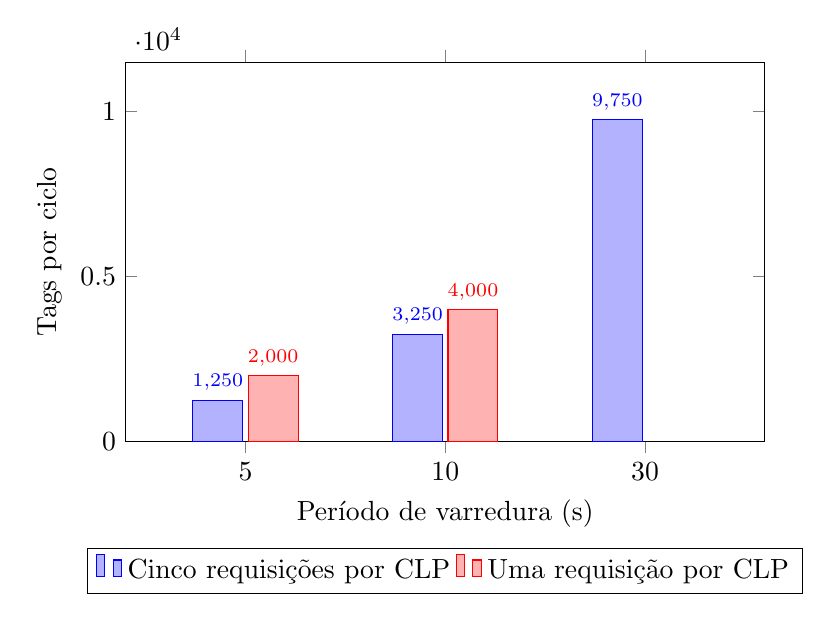
\begin{tikzpicture}
        \begin{axis}[
            ybar, width=0.8\textwidth, height=6.4cm,
            symbolic x coords={5,10,30},
            xtick=data,
            xlabel={Período de varredura (s)},
            ylabel={Tags por ciclo},
            ymin=0, ymax=11500, bar width=18pt, enlarge x limits=0.3,
            nodes near coords,
            every node near coord/.append style={font=\scriptsize},
            legend style={at={(0.5,-0.28)}, anchor=north, legend columns=2},
        ]
            \addplot coordinates {(5,1250) (10,3250) (30,9750)};
            \addplot coordinates {(5,2000) (10,4000)};
            \legend{Cinco requisições por CLP, Uma requisição por CLP}
        \end{axis}
    \end{tikzpicture}
    \vspace{0.2cm} \\
    Fonte: Autor.
\end{figure}

\subsubsection{Ensaio ponta a ponta com o servidor de teste}

\par Para validar a cadeia completa, o autor usou o ProtoProbe, um servidor Modbus de teste na porta 502, com identificador de escravo 1 e 2.500 registradores de retenção de 16 bits. Cadastraram-se, pela interface, uma planta, um dispositivo, uma tag no endereço 7, lida de 1 em 1 s, um dispositivo interno com uma tag gravável, um evento que compara a tag lida com um limite e um \emph{script} que copia o valor para a tag interna. Nenhuma função de escrita Modbus foi usada nessa prova.

\par O valor 12.314, mantido no endereço 7, chegou ao valor atual com qualidade boa. O evento disparou, o \emph{script} executou no contêiner isolado em 13 a 87 ms e gravou a tag interna com o mesmo valor, sem falha. Movendo o limite do evento, o \emph{script} executou nas duas transições. A prova mostra que a leitura Modbus, o valor atual, o detector de eventos, o motor de scripts e a escrita em tag interna funcionam em sequência, sem código específico do equipamento (RNF08).

\par O ensaio de carga contra o ProtoProbe cadastra um número crescente de tags, com períodos de 1 e de 5 s, e confere se as leituras gravadas coincidem com o esperado, se o valor atual acompanha as mudanças e se a lista de acompanhamento exibe o valor com o atraso previsto. A Tabela~\ref{tab:cap7_protoprobe} reserva o espaço para os resultados.

{\renewcommand{\arraystretch}{1.3}\small
\begin{xltabular}{\textwidth}{cccccc}
        \caption{Ensaio de carga de leitura contra o ProtoProbe.}
        \label{tab:cap7_protoprobe}\\
        \hline
        \textbf{Tags} & \textbf{Período} & \textbf{Duração} & \textbf{Leituras gravadas} & \textbf{Atraso até o Redis} & \textbf{Atraso até a tela} \\
        \hline
        \endfirsthead
        \hline
        \textbf{Tags} & \textbf{Período} & \textbf{Duração} & \textbf{Leituras gravadas} & \textbf{Atraso até o Redis} & \textbf{Atraso até a tela} \\
        \hline
        \endhead
        \endfoot
        \multicolumn{6}{c}{Fonte: Autor.} \\
        \endlastfoot
        10 & 1 s & a medir & a medir & a medir & a medir \\
        \hline
        50 & 1 s & a medir & a medir & a medir & a medir \\
        \hline
        100 & 5 s & a medir & a medir & a medir & a medir \\
        \hline
        500 & 5 s & a medir & a medir & a medir & a medir \\
        \hline
\end{xltabular}}

\todo[inline]{Medir: ensaio de carga de leitura contra o ProtoProbe (porta 502, escravo 1, 2.500 registradores). Não há número de vazão contra o ProtoProbe nos documentos do código, só a prova funcional da cadeia (specs/049-scripts-em-javascript/prova-protoprobe.md) e a campanha de capacidade com o simulador do repositório. Escolher o número de tags e os períodos da tabela, a duração (sugestão: 10 minutos por linha), e como medir o atraso até a tela (carimbo da leitura contra o instante em que o valor aparece).}

\subsection{Resultados da bancada}

\par A bancada reúne um \sigla{clp} que atua como servidor Modbus, um inversor de frequência que aciona um motor real, comandado pelo \sigla{clp} por rede serial \cite{SCHNEIDER_ATV320_MODBUS_MANUAL}, e o servidor do sistema. Os ensaios E1 a E6, na Tabela~\ref{tab:cap7_ensaios}, percorrem a operação do motor, que os professores repetem pelo tablet na demonstração. Duas medidas interessam: o tempo entre a confirmação do comando e a resposta do equipamento, que mede a latência do caminho de escrita, e o atraso do supervisório, entre uma mudança no equipamento e sua exibição na tela, limitado pela soma do período de varredura, do período de atualização da tela e de uma margem de processamento (RNF01).

\todo[inline]{Os ensaios E1 a E6 seguem o roteiro do Capítulo 6 (bancada: CLP TM221 e inversor ATV320). Conferir os parâmetros citados (referência de 40 e 30 Hz, rampas do inversor, limite de corrente) se o Capítulo 6 mudar, e preencher as tabelas e os gráficos com as medições.}

{\renewcommand{\arraystretch}{1.3}\small
\begin{xltabular}{\textwidth}{cXX}
        \caption{Ensaios da bancada.}
        \label{tab:cap7_ensaios}\\
        \hline
        \textbf{Id} & \textbf{Ensaio} & \textbf{Requisitos verificados} \\
        \hline
        \endfirsthead
        \hline
        \textbf{Id} & \textbf{Ensaio} & \textbf{Requisitos verificados} \\
        \hline
        \endhead
        \endfoot
        \multicolumn{3}{c}{Fonte: Autor.} \\
        \endlastfoot
        E1 & Leitura contínua com o motor desligado & RF01, RF02, RF03, RF04, RNF01 \\
        \hline
        E2 & Partida pelo supervisório & RF06, RF08, RNF01 \\
        \hline
        E3 & Parada pelo supervisório & RF06, RF08, RF17, RNF01 \\
        \hline
        E4 & Alarme de corrente alta e reconhecimento & RF16, RF17, RNF05 \\
        \hline
        E5 & Perda de comunicação e retorno & RF01, RF03, RF16 \\
        \hline
        E6 & Troca da referência de frequência & RF06, RF08, RNF05 \\
        \hline
\end{xltabular}}

\par \emph{Ensaio E1.} Com o motor parado, as grandezas não variam, o que isola o desempenho da aquisição. O ensaio mantém as tags em leitura contínua e confere se o histórico não perde amostras, se o carimbo de tempo é monotônico e espaçado pelo período configurado, com variação de poucos milissegundos, e se a lista de acompanhamento atrasa no máximo o período de varredura mais o de atualização da tela. Espera-se uma taxa de entrega próxima de 100\,\% e nenhum alarme.

\par \emph{Ensaio E2.} O operador define a referência de 40 hertz e envia o comando de partida pelas quatro fases. O sistema escreve a ordem em um registrador do \sigla{clp}, que a repassa ao inversor. O ensaio mede o tempo entre a confirmação e a resposta do \sigla{clp}, em que o comando é dado como concluído, e o tempo até a frequência começar a subir na tela. Espera-se a resposta em dezenas de milissegundos, bem abaixo do limite de 30 s do comando, que a trava por tag impeça um segundo comando simultâneo e que o comando fique registrado com o operador, a tag, o valor e o instante.

\par \emph{Ensaio E3.} A ordem de parada segue o mesmo caminho, e a frequência desce pela rampa de desaceleração. Espera-se o mesmo tempo de comando do E2, que a tela acompanhe a frequência até zero e que a leitura continue sem perda, sem alarme de comunicação, o que separa o efeito do processo do efeito do sistema.

\par \emph{Ensaio E4.} Com o motor ligado, a corrente cruza o limite configurado [A CONFIRMAR] do alarme de corrente alta, e o detector cria uma ocorrência. O ensaio mede o tempo entre o cruzamento e a exibição no indicador de alarmes, que deve ser da ordem do atraso do supervisório. O operador reconhece o alarme, e confere-se que o registro guarda o nome e o instante. Parado o motor, a corrente cai abaixo do limite, descontada a banda morta, e o alarme retorna ao normal. Espera-se um alarme único por cruzamento e a sequência correta na linha do tempo.

\par \emph{Ensaio E5.} A comunicação é interrompida desconectando o cabo Ethernet entre o comutador e o \sigla{clp}, e depois restabelecida. Durante a falha, o \sigla{clp} continua executando o programa. O sistema marca o valor como desatualizado depois de três períodos de varredura, mantendo o último valor e o carimbo, e o dispositivo passa a degradado depois de três ciclos falhos. Com o cabo de volta, o primeiro ciclo bem-sucedido fecha o estado, sem rajada de leituras acumuladas. O ensaio mede o tempo até a marcação de desatualizado e o tempo até a volta à qualidade boa e confere que não há lacuna preenchida no histórico, pois a lacuna é a evidência da falha.

\par \emph{Ensaio E6.} Com o motor a 40 hertz, o operador altera a referência para 30 hertz pelo mesmo comando. O ensaio mede o tempo até a resposta do \sigla{clp} e até a frequência atingir a referência, e confere que um segundo comando imediato é recusado pela trava por tag e que o reenvio com a mesma chave de idempotência não cria uma segunda escrita.

\par A Tabela~\ref{tab:cap7_medidas} reúne as medidas previstas.

{\renewcommand{\arraystretch}{1.3}\small
\begin{xltabular}{\textwidth}{cXcc}
        \caption{Medidas previstas nos ensaios da bancada.}
        \label{tab:cap7_medidas}\\
        \hline
        \textbf{Ensaio} & \textbf{Medida} & \textbf{Esperado} & \textbf{Medido} \\
        \hline
        \endfirsthead
        \hline
        \textbf{Ensaio} & \textbf{Medida} & \textbf{Esperado} & \textbf{Medido} \\
        \hline
        \endhead
        \endfoot
        \multicolumn{4}{c}{Fonte: Autor.} \\
        \endlastfoot
        E1 & Taxa de leituras gravadas em relação às esperadas & acima de 99\,\% & a medir \\
        \hline
        E1 & Variação do intervalo entre carimbos consecutivos & poucos ms & a medir \\
        \hline
        E1 & Atraso do supervisório (equipamento até a tela) & varredura mais atualização da tela & a medir \\
        \hline
        E2 & Confirmação do operador até a resposta do CLP à escrita & dezenas de ms & a medir \\
        \hline
        E2 & Resposta do CLP até a primeira mudança de frequência na tela & varredura mais atualização da tela & a medir \\
        \hline
        E2 & Duração da rampa de aceleração observada & valor configurado no inversor & a medir \\
        \hline
        E3 & Confirmação do operador até a resposta do CLP à escrita & dezenas de ms & a medir \\
        \hline
        E3 & Resposta do CLP até a frequência zero na tela & rampa de desaceleração mais atraso do supervisório & a medir \\
        \hline
        E3 & Leituras perdidas durante a transição & nenhuma & a medir \\
        \hline
        E4 & Cruzamento do limite até o alarme na tela & varredura mais atualização da tela & a medir \\
        \hline
        E4 & Ocorrências geradas por cruzamento & uma & a medir \\
        \hline
        E4 & Reconhecimento até o registro com nome e instante & imediato (próxima atualização da tela) & a medir \\
        \hline
        E5 & Interrupção até a marcação de desatualizado & três períodos de varredura & a medir \\
        \hline
        E5 & Interrupção até o estado de comunicação degradado & três ciclos falhos & a medir \\
        \hline
        E5 & Retorno do cabo até a qualidade boa na tela & um ciclo mais atualização da tela & a medir \\
        \hline
        E5 & Linhas gravadas no histórico durante a falha & nenhuma & a medir \\
        \hline
        E6 & Confirmação do operador até a resposta do CLP à escrita & dezenas de ms & a medir \\
        \hline
        E6 & Resposta do CLP até a frequência medida igual à referência & rampa do inversor mais atraso do supervisório & a medir \\
        \hline
        E6 & Segundo comando imediato na mesma tag & recusado pela trava & a medir \\
        \hline
        E6 & Reenvio com a mesma chave de idempotência & uma única escrita & a medir \\
        \hline
\end{xltabular}}

\todo[inline]{Medir e inserir, para cada ensaio, o gráfico da tela e os valores da Tabela~\ref{tab:cap7_medidas}. Informar as rampas do inversor, o registrador da referência, o período de varredura, a corrente em cada regime e a linha do registro de comandos. Confirmar a referência de 40 e 30 Hz e se o alarme de falha de comunicação foi ligado.}

\subsection{Validação dos requisitos}

\par A Tabela~\ref{tab:cap7_requisitos} confronta cada requisito com a evidência disponível. É atendido o requisito com medida realizada ou teste automatizado, e parcialmente atendido o que depende da bancada ou de uma medida ainda não feita, caso dos requisitos de comando, de alarmes e de atraso, que dependem dos ensaios E1 a E6. Nenhum requisito ficou sem evidência.

{\renewcommand{\arraystretch}{1.3}\small
\begin{xltabular}{\textwidth}{cXc}
        \caption{Validação dos requisitos.}
        \label{tab:cap7_requisitos}\\
        \hline
        \textbf{Id} & \textbf{Evidência} & \textbf{Situação} \\
        \hline
        \endfirsthead
        \hline
        \textbf{Id} & \textbf{Evidência} & \textbf{Situação} \\
        \hline
        \endhead
        \endfoot
        \multicolumn{3}{c}{Fonte: Autor.} \\
        \endlastfoot
        RF01 & Testes do driver, ensaio contra o ProtoProbe, campanha de capacidade até 9.750 tags a 30 s, E1 & Atendido \\
        \hline
        RF02 & Testes de gravação e de partição, teste de carga do histórico (até 9.400 linhas por segundo), E1 & Atendido \\
        \hline
        RF03 & Teste de carga de valores atuais de 10 minutos, E1 & Atendido \\
        \hline
        RF04 & Testes automatizados do carimbo por ciclo, E1 & Atendido \\
        \hline
        RF05 & Testes de login, troca de senha, cargos, grupos e permissões & Atendido \\
        \hline
        RF06 & Testes da cadeia de comando, prova do comando contra o ProtoProbe, E2, E3 e E6 & Parcial \\
        \hline
        RF07 & Testes e conferência visual do evento agendado com \emph{script} que escreve & Atendido \\
        \hline
        RF08 & Testes da trava por tag, da idempotência e do registro de comandos, E2 e E6 & Parcial \\
        \hline
        RF09 & Testes de recarga do cadastro sem reinício da aquisição & Atendido \\
        \hline
        RF10 & Testes do cadastro, do esquema e das pastas de tags & Atendido \\
        \hline
        RF11 & Testes das variáveis derivadas e das tags internas, teto medido por contêiner & Atendido \\
        \hline
        RF12 & Medidas do motor isolado, testes de isolamento, prova do \emph{script} contra o ProtoProbe & Atendido \\
        \hline
        RF13 & \emph{Lighthouse} da tela de dashboard, testes, E1 & Atendido \\
        \hline
        RF14 & Medida de 8 ms para aplicar um ciclo no sinótico, \emph{Lighthouse}, conferência visual & Atendido \\
        \hline
        RF15 & Testes do mapa e das consultas de tendência ao histórico, E3 & Atendido \\
        \hline
        RF16 & Testes dos detectores e das ocorrências, E4 e E5 & Parcial \\
        \hline
        RF17 & Testes da linha do tempo, do registro de comandos e de alarmes, E4 & Atendido \\
        \hline
        RNF01 & Medida do lado do cliente, teste de carga de valores atuais, atraso do supervisório em E1 a E6 & Parcial \\
        \hline
        RNF02 & Medida do teto por réplica, dispositivo fixo em uma réplica, sem medida com duas réplicas & Parcial \\
        \hline
        RNF03 & Testes de reconstrução do Redis e de filas duráveis, sem ensaio de queda de réplica & Parcial \\
        \hline
        RNF04 & Testes de permissão, teste de segurança de fim de lote & Atendido \\
        \hline
        RNF05 & Testes de limite de requisições, de trava por tag e de registro de comando e de reconhecimento & Atendido \\
        \hline
        RNF06 & Testes de isolamento do motor de scripts, medidas de custo e de memória & Atendido \\
        \hline
        RNF07 & Testes da cifra de segredos com AES-256-GCM & Atendido \\
        \hline
        RNF08 & Mesma configuração Modbus com o ProtoProbe, os simuladores e o CLP da bancada & Atendido \\
        \hline
        RNF09 & Formato \sigla{json} verificado por teste & Atendido \\
        \hline
        RNF10 & Serviços independentes ligados por Moleculer e filas, guardas de arquitetura & Atendido \\
        \hline
        RNF11 & Pilha completa de contêineres com limites de recursos, usada em todas as medidas & Atendido \\
        \hline
        RNF12 & Acesso por navegador, \emph{Lighthouse} em celular, interface em português & Atendido \\
        \hline
\end{xltabular}}

\subsection{Qualidade de software}

\par A qualidade do código faz parte do resultado, porque um supervisório que mexe em equipamentos precisa ser verificável. O repositório reúne cerca de 3.600 arquivos de teste, dos quais cerca de 3.000 são unitários, mais de 600 são de integração, com o banco e o Redis reais, e 17 são de carga. O código das camadas de domínio e de aplicação tem cobertura exigida de 100\,\% de linhas e de ramos.

\par Verificações automáticas rodam sobre o repositório inteiro e reprovam violações de projeto, como uma camada que depende de outra fora da ordem permitida ou um arquivo sem teste. O fim de cada lote de trabalho executa a análise estática, a verificação de tipos, os testes, a auditoria de dependências, um teste de segurança do tipo caixa preta e uma revisão independente do código. Esse roteiro é executado localmente, pois ainda não há integração contínua em servidor.

\todo[inline]{Os números de arquivos de teste são contagens aproximadas dos arquivos versionados no repositório do código (sem rodar os testes). Se quiser números de testes executados e de cobertura, é preciso rodar a suíte e inserir o resultado. Confirmar também se vale citar a revisão adversarial no texto.}

\subsection{Limitações e comparação com a literatura}

\par Os resultados têm cinco limitações. As medidas saem de um computador compartilhado, sem rede entre os contêineres, e os tetos variaram até 50\,\% entre execuções. A carga foi gerada por simuladores que respondem em 5 ms, sem o tempo de modems e redes industriais. O efeito de réplicas não foi medido. A execução em mais de um servidor não foi implantada. E o contêiner de \emph{workers} ficou abaixo do piso planejado para variáveis derivadas e tags internas, o próximo alvo de otimização.

\par O \sigla{scada} de baixo custo desenvolvido em C\# com um \sigla{clp} comercial e testado em uma planta de alimentos valida o funcionamento em campo, mas não relata latência nem vazão do software \cite{PHUYAL2020_COST_EFFICIENT_SCADA}. O presente trabalho segue a mesma motivação e acrescenta uma avaliação quantitativa, ainda que em laboratório. Já a dissertação sobre um supervisório baseado na web compara tempo de resposta, carga de processador e tráfego de rede \cite{AHMED2011_EFFICIENT_WEB_SCADA}. A diferença aqui é a arquitetura, que separa a aquisição, o \emph{cache} e o histórico em contêineres independentes e torna cada gargalo mensurável isoladamente.
